\documentclass[a4paper,12pt]{book}

\usepackage{amsmath,amsthm,amssymb}
\usepackage{mathtext}
\usepackage[T1,T2A]{fontenc}
\usepackage[utf8]{inputenc}
\usepackage[ukrainian]{babel}
\usepackage{graphicx}
\usepackage{wasysym}
\usepackage[dvipsnames]{xcolor}
\usepackage{multicol}
\usepackage{hyperref}


\newcounter{problem}[chapter]
\newcommand{\problem}{%
    \medskip\medskip%
    \par\noindent\addtocounter{problem}{1}%
    \textbf{\large\color{Bittersweet}\arabic{chapter}.\arabic{problem}. }%
}

\newcommand{\problemname}[1]{\textbf{#1}.}

\newenvironment{dialogue}{%
    \medskip%
    \list{--}{\itemsep=\parskip \topsep=\parskip \parsep=\parskip}%
}{
    \endlist%
    \medskip%
}

\renewcommand{\arraystretch}{1.5}


\begin{document}

\author{
    Сашко Петров\\
    \texttt{alexandervpetrov@gmail.com}
    \and
    Валентина Мержиєвська\\
    \texttt{yakavoska@gmail.com}
}
\title{\Huge $4 \times 40$}
\date{2 грудня 2015}

\frontmatter
\maketitle
\tableofcontents
\mainmatter
\chapter*{Передмова}

Це не підручник з математики, не робочий зошит.
Це лише збірка завдань з математики, які ми вигадували для дітей
в початкових класах БеркоШко.
Звісно не всі, по 40 за кожний рік.

Можливо колись вдасться написати й підручник з математики,
який буде яскравим і захопливим.
Більше схожим на якісні підручники з іноземної мови, з дотепними персонажами,
живими малюнками, цікавими завданнями, з додатковою методичкою для вчителя.
Але наразі хочеться поділитися вже тим, що маємо.
Бо поки система освіти буде реформована, поки з’являться підручники
нового покоління, діти вже виростуть.

Частина цих завдань була всерйоз продумана наперед,
частина – вигадана на хочу під час заняття:
\begin{dialogue}
\item Ну й про кого ви б хотіли сьогодні задачку?
\item Про зелених хробачків!
\item Ну гаразд. Одного дня\ldots
\end{dialogue}

Окрім завдань із одним рішенням, ми свідомо іноді давали дітям завдання,
які не мають розв’язку, або мають кілька можливих відповідей.

Надихайтесь, навчайтесь з легкістю, грайтесь в математику,
експериментуйте й творіть. \smiley

\medskip

{ \emph{Оскільки завдання публікуються вперше, то прохання до читачів,
якщо раптом будуть знайдені помилки,
повідомити про це на електронну пошту\footnote{
    E-mail: \texttt{many.pure@gmail.com}
}.
Також будемо вдячні за відгуки}} \smiley

\chapter{Перший клас}


\problem
Намалюй на аркушах у~клітинку:
\begin{enumerate}
    \item трикутник, у~якого дві сторони однакові;
    \item трикутник, одна сторона якого займає 4~клітинки, а~друга~---
    2~клітинки;
    \item чотирикутник, у~якого всі сторони однакові;
    \item чотирикутник, у~якого всі сторони однакові, але не~квадрат;
    \item квадрат, який складається з~чотирьох клітинок;
    \item ще чотири квадрати, щоб кожен наступний був більший від попереднього;
    \item всередині кожного з~отриманих квадратів намалюй коло.
    Намагайся, щоб кола були якомога більшими,
    але все одно залишалися всередині квадратів.
\end{enumerate}


\problem
% TAGS: many_solutions
На нелінованому аркуші намалюй два кола (червоне та зелене)
і три цифри («один», «три», «п'ять») так,
щоб усе наступне було правдою:
\begin{itemize}
    \item цифри «один» та «п'ять» розташовані всередині червоного кола;
    \item цифри «п'ять» та «три» розташовані всередині зеленого кола;
    \item цифра «один» розташована ззовні зеленого кола.
\end{itemize}


\problem
Перед початком перерви у~Маші було шість яблук,
у~Іванки~--- чотири яблука, а~у~Федька~--- два яблука.
Це можна скорочено записати (намалювати), наприклад, так:

\begin{center}
\sffamily
\begin{tabular}{rccc}
  & \sffamily Маша & Іванка & Федько \\
  Спочатку: & 6 & 4 & 2 \\
\end{tabular}
\end{center}

Потім відбулися такі події:
\begin{enumerate}
    \item Маша дала одне яблуко Федьку;
    \item Іванка з'їла два яблука;
    \item Федько дав два яблука Іванці;
    \item Маша з'їла три яблука;
    \item Іванка віддала три яблука Федьку;
    \item Маша з'їла одне яблуко.
\end{enumerate}

Відтак перерва скінчилась і~всі пішли на наступне заняття.
Запиши (намалюй) на окремому аркуші, що відбувалося з~яблуками
та учнями протягом перерви.

Як ти думаєш:
\begin{itemize}
    \item Скільки всього було яблук на початку?
    \item Скільки всього яблук мали Іванка, Маша та Федько
    після закінчення перерви?
    \item Скільки яблук з'їли учні?
    \item Хто найменше зголоднів перед перервою? Чому?
    \item Хто найбільше зголоднів перед перервою? Чому?
\end{itemize}


\problem
Роздивися малюнок:

\begin{figure}[ht]
    \centering
    
\includegraphics[width=0.8\textwidth]{1-04-1}
\end{figure}

Чи правда, що:
\begin{enumerate}
    \item всередині овалу розташовані два квадрата?
    \item ззовні кола розташовані два прямокутника?
    \item на малюнку зображено один ромб?
    \item ззовні овалу розташований квадрат?
    \item всередині овалу можна знайти три ромби?
    \item всередині фігури без кутів можна знайти прямокутник?
    \item всі фігури на малюнку різні?
\end{enumerate}



\problem
Що буде далi? Чому?
Спробуй знайти принаймнi два наступних числа (двi літери).
\begin{enumerate}
    \item 13, 15, 17, 19, \ldots
    \item 20, 17, 14, 11, \ldots
    \item 1, 1, 2, 1, 3, 1, 4, 1, \ldots
    \item 1, 1, 2, 3, 3, 5, 4, 7, \ldots
    \item 1, 2, 4, 7, 11, 16, \ldots
    \item 1, 1, 2, 3, 5, 8, 13, \ldots
    \item 1, 2, 4, 8, 16, \ldots
    \item А, В, Г, Д, Е, Ж, З, І, Ї, \ldots
    \item I, К, Н, Р, \ldots
    \item П, М, Й, И, \ldots
    \item Г, Ґ, Ж, З, Й, К, О, П, \ldots
    % в наступній послідовності літери топологічно еквівалентні
    \item Г, Ґ, И, І, Л, \ldots
\end{enumerate}


\problem
Маєш 5~шашок. Дві з них чорні, решта~--- білі.
Розташуй їх у рядочок всіма можливими способами, але так,
щоб послідовності не повторювалися.
Рішення замалюй у~зошиті.


\problem
Федько, Маша й~Іванка мешкають в~одному будинку.
Маша~--- на п’ятому поверсі, Федько~--- на 2~поверхи вище,
а~Іванка~--- одразу над Федьком.
На якому поверсі мешкає Іванка?
Скільки поверхів між помешканнями Маші й~Іванки?


\problem
% TAGS: discussion
\problemname{Теорія ймовірностей}
\begin{enumerate}
    \item В~шафці дві пари гумових чобітків різного кольору
    (або: в~мішечку 4~кубики, по 2~двох різних кольорів).
    Ти збираєшся на прогулянку і~хочеш взути пару чобітків однакового кольору,
    але дістаєш їх із~шафки наосліп. Чи пощастить?
    \item На поличці три пари рукавичок різного кольору
    (в мішечку 6~кубиків, по 2~трьох різних кольорів).
    А~тепер підбираємо однакову пару рукавичок.
    Чи вдасться піти на прогулянку в~однакових рукавичках?
\end{enumerate}


\problem
% TAGS: discussion
\problemname{Гра «Бігові доріжки»}
Є поле в~клітинку, рядки пронумеровані від~1 до~14.
Кожний розставляє свої фішки на ці «бігові доріжки».
Далі підкидають 2~гральних кубика, обчислюють суму крапочок,
які випали на гранях кубиків, і~фішка на доріжці з~таким номером
робить крок уперед.
Виграє та фішка, яка першою «добіжить» до фініша.

\emph{%
Суму чисел у~грі діти рахують блискавично.
Цікаво обговорювати чому фішки, які стоять на доріжках~2, 13, 14, рухаються повільно,
а~та, що на доріжці~1~--- взагалі не може зрушити з~місця.
}


\problem
\problemname{Топологічна абетка}

\begin{figure}[ht]
    \centering
    \quad \quad
    \begin{subfigure}{0.3\textwidth}
        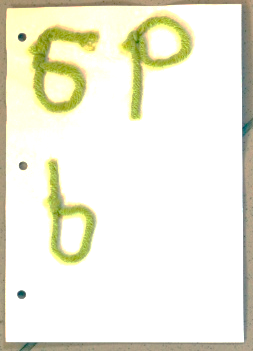
\includegraphics{1-10-1-a}
    \end{subfigure}
    \begin{subfigure}{0.3\textwidth}
        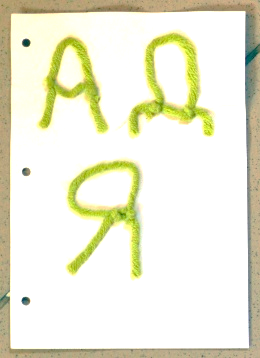
\includegraphics{1-10-2-a}
    \end{subfigure}
    \begin{subfigure}{0.3\textwidth}
        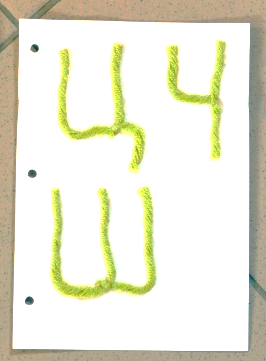
\includegraphics{1-10-3-a}
    \end{subfigure}
\end{figure}

\begin{enumerate}
    \item Знайди всі українські й англійські літери, цифри
    та математичні символи, які можна виготовити з~одного шматка мотузки.
    \item Знайди всі літери, цифри та математичні символи,
    які можна виготовити з~кільця з~одним «вусиком»;
    \item Знайди всі літери, цифри та математичні символи,
    які можна виготовити з~кільця з~двома «вусиками»;
    \item Знайди всі літери, цифри та математичні символи,
    які можна виготовити з~просто кільця («безвусого»)
    \item Знайди всі букви, цифри та математичні символи,
    які можна виготовити з~мотузочки з~язичком посередині,
    тобто вузлика з~трьома хвостиками.
\end{enumerate}

\emph{%
«Заготовку» (коло з~певною кількістю вусиків) можна як завгодно вигинати,
але не можна розривати і~зв'язувати кінці.
Накладати мотузку саму на себе або клеїти вздовж,
утворюючи лінії товщиною в~дві мотузки, також не можна.
}


\problem
На правій шальці терезів 4~камінчика і~ще 5~камінчиків,
а~на лівій~--- 3~камінчика і~ще~7.
Яка шалька терезів опуститься нижче?

\emph{%
Для задач на зважування у першому класі бажано використовувати
камінчики, однакові за розміром і~вагою.
Терези і~камінчики~--- не намальовані, а~справжні.
Задачу слід вирішувати на матеріальних об’єктах,
в~зошит замальовувати вже готове рішення.
}


\problem
% TAGS: many_solutions
Намалюй фігури:
\begin{enumerate}
    \item Намалюй трикутник, п'ятикутник, ромб і~коло так,
    щоб усе наступне було правдою:
    \begin{itemize}
        \item трикутник розташований всередині кола;
        \item ззовні кола немає ромба;
        \item п'ятикутник намальований навколо трикутника.
    \end{itemize}
    \item Намалюй на аркуші в~клітинку два трикутники,
    два чотирикутники і~коло так, щоб усе наступне було правдою:
    \begin{itemize}
        \item один чотирикутник рівно вдвічі більший за інший;
        \item трикутник знаходиться всередині кола;
        \item коло розташоване всередині трикутника;
        \item на малюнку немає квадратів.
    \end{itemize}
    \item Намалюй два чотирикутника, коло і~п'ятикутник так,
    щоб усе наступне було правдою:
    \begin{itemize}
        \item ромб знаходиться всередині п'ятикутника;
        \item коло розташоване навколо п'ятикутника;
        \item всередині прямокутника намальоване коло.
    \end{itemize}
    \item Напиши слово «МАТЕМАТИКА» і~намалюй два кола так,
    щоб букви «К» і~«Т» знаходилися в~різних колах,
    а~букву «М» можна було знайти всередині двох кіл одночасно.
\end{enumerate}


\problem
Завдання з терезами.
\begin{enumerate}
    \item На правій шальці терезів 10~камінчиків, а на лівій~---
    5~камінчиків і~ще~5. Яка шалька терезів опуститься нижче?
    \item З~правої шальки взяли 2~камінчики і~переклали на ліву.
    Яка шалька нижче?
\end{enumerate}
Запиши відповіді математичною мовою, застосовуючи цифри
та позначки «$=$», «$<$», «$>$».


\problem
Відтвори на терезах таку історію: $7+9 < 10+8$.


\problem
Розбий фігуру на 4~однакові частини:

\begin{figure}[ht]
    \centering
    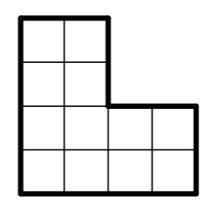
\includegraphics{1-15-1}
\end{figure}


\problem
Запиши речення математичною мовою~--- користуючись цифрами,
позначками дій («$+$» або «$-$») та знаками порівняння («$<$», «$>$», «$=$»):
\begin{enumerate}
    \item Шістнадцять і~дев'ять буде двадцять п'ять.
    \item Якщо від десяти забрати три, то вийде шість.
    \item Десять кісточок можна скласти з двох однакових купок~---
    по п'ять кісточок у~кожній.
    \item Два олівці в~лівій кишені та~ще чотири у~правій,
    разом виходить менше ніж шість олівців.
\end{enumerate}
Чи не здалося тобі щось дивним у~деяких з~цих речень?

\problem
Завдання з~терезами:
\begin{enumerate}
    \item У~ліву шальку терезів поклали чотири і~п'ять кісточок,
    а~в~праву шальку~--- три кісточки і~потім ще сім.
    Намалюй, як виглядатимуть терези.
    Одразу після цього запиши, що відбулося з~терезами,
    але математичною мовою.
    \item У~лівій шальці терезів лежить десять кісточок,
    а~у~правій~--- чотири кісточки.
    Намалюй, як виглядатимуть терези. Запиши математичною мовою.

    Коли у~праву шальку поклали камінець терези врівноважились.
    Намалюй, як виглядають терези зараз.
    Запиши математичними символами
    (замість камінця напиши знак питання «?» в~кружечку).
    Як ти думаєш, скільки кісточок важить камінець? Чому?
\end{enumerate}


\problem
Намалюй квадрат:
\begin{enumerate}
    \item кожна сторона якого проходить вздовж двох клітинок;
    \item у~два рази більший за перший;
    \item в~три рази більший за перший.
\end{enumerate}
Для кожної фігури підпиши довжини сторін.


\problem
Розкодуй слово:
\begin{enumerate}
    \item 10 11 17 1;
    \item 17 1 23 7 17 1 23 11 15 1;
    \item 27 24 15 7 21 15 1;
    \item 20 7 21 7 21 3 1.
\end{enumerate}

\emph{%
Ключ до коду~--- порядковий номер літери в~абетці, тільки це таємниця.
}


\problem
Назви числа:
\begin{enumerate}
    \item по порядку за зростанням, починаючи з~випадкового числа
    в~межах $1\ldots30$;
    \item по порядку за спаданням;
    \item через одне за зростанням;
    \item через одне за спаданням.
    \item Яке третє число після 17, якщо рахувати через одне?
    \item Яке число на два випереджає 23?
\end{enumerate}


\problem
% TAGS: many_solutions
У~Марка було 6~яблук. З~них 3~були зелені, а~решта~--- червоні.
У~Іванки червоних яблук було на~2 більше, ніж у~Марка,
а~зелених~--- зовсім не було.
У~Машки було стільки~ж яблук, як і~в~Іванки.
Але були і~червоні, і~зелені. Зелених було більше.
А~у~Федька було стільки~ж зелених яблук, скільки й~у~Марка,
а~червоних~--- стільки~ж, скільки й у~Машки.
Запитання: скільки яблук було у~Федька?


\problem
% TAGS: many_solutions
Їжачок знайшов 10~яблук.
Більшу частину з~них він віддав знайомому зайцю.
Скільки яблук могло залишитись у~нього?


\problem
Запиши математичною мовою та знайди невірні (неправдиві) речення:
\begin{enumerate}
    \item Два, п'ять, сім і три~--- разом буде сімнадцять.
    \item Якщо від сімнадцяти забрати сім, то залишиться десять.
    \item Дівчинка з'їла три абрикоси вранці, а~потім чотири на обід
    і~ще дві~--- ввечері. Отже, за день вона з'їла дев'ять абрикос.
    \item В~помаранчевому мішечку лежало чотири кісточки,
    а~в~синьому~--- п'ять кісточок. Разом у~мішечках~--- дев'ять кісточок.
    \emph{Завдання з~хитринкою. В~одному випадку відповідь правдива,
    а~в~іншому~--- ні (мішечки можуть бути заховані один в~одний).}
    \item Мама купила два десятки яєць, а~потім почала робити з~них омлети.
    Щоранку вона робила омлет із~трьох яєць.
    На скільки омлетів вистачить куплених яєць? А~скільки яєць ще залишиться?
\end{enumerate}


\problem
% TAGS: many_solutions
Скільки?
\begin{enumerate}
    \item Скільки разів треба розрізати мотузочку, щоб вийшло 5~шматочків?
    Спробуй відповісти подумки, а~потім намалюй і~перевір.
    \item Скільки вузликів потрібно, щоб зв'язати 7~мотузок в~одну довгу?
    Спробуй порахувати усно, а~потім намалюй і~перевір.
    \item Скільки треба зробити розрізів, щоб перетворити кільце
    на 5~шматочків? Спробуй відповісти усно, а~потім намалюй і~перевір.
    \item Всередині синього кола три трикутника, а~всередині зеленого кола
    трикутників п'ять. Скільки всього трикутників може бути на малюнку?
    \item Хтось на мотузочці зав'язав два більших і~два менших вузлика.
    А~всього вузликів три. Спробуй здогадатися, як таке могло статися? Намалюй.
\end{enumerate}


\problem
Вгадай число:
\begin{enumerate}
    \item Я задумав число. Потім додав до нього 5. Вийшло 17.
    Яке число я задумав?
    \item Я задумав число. Потім додав до нього 5.
    Потім від того, що вийшло відняв 3. Вийшло 2.
    Яке число я задумав?
\end{enumerate}


\problem
% TAGS: discussion
Як ти вважаєш, які з~речень є правдивими? Чому?
А~які інколи бувають правдою, а~інколи неправдою? Поясни. Наведи приклади.
А~які з~речень на твою думку є неправдивими? Поясни. Виправ помилки.
\begin{enumerate}
    \item П'ять і~сім разом~--- це стільки~ж, скільки буде два рази по шість.
    \item Сімнадцять кісточок можна скласти з~трьох рядів
    по шість кісточок в~кожному.
    \item Тиждень складається з~7~днів.
    \item Місяць (той, що у календарі) складається з~30~днів.
    \item Квадрат можна назвати чотирикутником.
    \item Чотирикутник можна назвати квадратом.
\end{enumerate}


\problem
Федько зібрав поїзд з~Lego. Поїзд тягнув тепловоз, а~за ним йшли вагони.
Один лісовоз, один поштовий вагон і~декілька пасажирських вагонів.
Пасажирських вагонів у~поїзді було найбільше.
Поїзд у Федька вийшов довгий~--- 1 метр і~5~сантиметрів.
Скільки пасажирських вагонів було у~поїзді,
якщо тепловоз має довжину 25~сантиметрів, а~всі вагони~--- по 20~сантиметрів.


\problem
З~початком весни на П'ятихатках почали танути бурульки.
Женька й~Андрій кожного ранку виходили на двір і~рахували, скільки розтануло,
а~скільки залишилось.
Першого березня розтануло чотири найменших бурульки.
Другого~--- перетворились на~воду ще п'ять.
У третій день весни зникло бурульок на дві менше, ніж у~перший.
Четвертого березня розтануло стільки~ж, скільки другого.
А~п'ятого березня зранку з~даху звисало лише дві.

З'ясуй скільки бурульок було на початку.
А~скільки їх було у~кожний зі згаданих днів?
Запиши математичною мовою, як змінювалася кількість бурульок
протягом спостережень.


\problem
% TAGS: many_solutions
Слон, мишеня, заєць та папуга вирішили позмагатися, хто швидше з'їде
з~гори на лижах. Вони піднялися на вершину гори й~одночасно рушили вниз.
Дізнайся, в~якому порядку вони дісталися фінішу, якщо відомо, що:
\begin{itemize}
    \item Мишеня їхало швидше за зайця.
    \item Папуга приїхав до підніжжя гори не третім і~не першим.
    \item Слон приїхав одразу після зайця.
\end{itemize}


\problem
Валя на Масляну напекла купу млинців і~після того, як пригостила всіх
і~сама поласувала, розклала ті, що залишилися, на дві тарілки порівну.
Млинці спокійно лежали на цих двох тарілках (лівій і~правій)
аж до закінчення заняття з~математики.
Потім прибігли учні разом із Сашком і~все з'їли.
Відомо, що Федько, Марко й~Іванка їли з~правої тарілки,
а~Машка із Сашком~--- з~лівої.
Також відомо що Марко з'їв 4~млинці, Іванка~--- 3,
Машка і~Федько з'їли млинців порівну, кожний на один млинець більше за Марка.

Скільки млинців з'їв Сашко?
Спробуй стисло намалювати все що відбулося із млинцями.
Подумай, як би ти записав цю історію математичною мовою?


\problem
На ліву шальку терезів поклали 3~камінці.
Перший важить стільки, скільки й 4~кісточки.
Вага другого становить шість кісточок.
А~третього додолу тягне так само, як 2~кісточки.
На правій шальці терезів було 7~кісточок.
Але після того, як на праву шальку ще прилетів іграшковий дракон,
терези врівноважились.

Визнач, з~якою силою тягне вниз іграшкового дракона,
що сидить на правій шальці.


\problem
Федько і~Василько пішли з~татком до лісу.
Там вони гуляли поміж дерев, слухали спів пташок,
збирали жолуді й~горішки ліщини.
Василькові дуже сподобалися жолуді, тому він набрав в~кишеню більше
жолудів, ніж ліщини. А~Федько збирав ліщину, жолуді брав рідко,
тому в~його кишені було більше горішків, ніж жолудів.
Але у~Федька кишені більші, ніж у~братика, тому вмістили
більше горішків і~жолудів, ніж у~Василька.

Скільки жолудів і~горішків ліщини назбирав кожний з~братиків,
якщо вдома, коли вони висипали з~усіх кишень на стіл свої знахідки,
татко нарахував 8~жолудів і~7~горішків ліщини.


\problem
% TAGS: discussion
Які з~наступних тверджень є правдою?
\begin{enumerate}
    \item Якщо коло знаходиться всередині трикутника,
    а~трикутник знаходиться всередині квадрата,
    то коло знаходиться всередині квадрата.
    \item Якщо жовта мотузочка довша за зелену,
    а~зелена довша за червону, то жовта довша за червону.
    \item Якщо яблуко важче за камінь, а~камінь важить більше за пінопласт,
    то яблуко важче за пінопласт.
    \item Якщо равлик швидший за зайця, а~заєць швидший за страуса,
    то равлик швидший за страуса.
\end{enumerate}
Подумай, як дуже стисло записати (замалювати) кожне з~тверджень.


\problem
На заняття прийшли троє учнів: Машка, Іванка і~Федько.
І~сіли за три парти: ліву, середню і~праву.
Скількома різними способами учні можуть вибрати собі парти?
Відшукай і~схематично намалюй всі можливі варіанти.
У~скількох з~них Іванка сидить поряд із Машкою?
Скільки існує варіантів розсаджування, де Машка сидить поряд із Федьком?
Чи можна учням сісти за парти так,
щоб Машка сиділа поряд із Федьком та Іванкою одночасно?



\problem
У твоїх~руках є дві мотузочки:
одна довжиною у~5~сірників, а~друга~--- у 8~сірників.
Більше нічого в~твоїх~руках немає (сірників теж).
\begin{enumerate}
    \item Як можна відміряти шматок мотузки довжиною у~3~сірники?
    \item Як можна відміряти шматок мотузки довжиною у~4~сірники?
    \item Як можна відміряти шматок мотузки довжиною в~1~сірник?
\end{enumerate}
Запиши кожний зі знайдених способів виготовлення математичною мовою.


\problem
Чи правда, що можна намалювати коло, всередині якого знаходиться
трикутник, не відриваючи олівця від паперу?
(Крім кола та трикутника, інших ліній на малюнку не повинно бути).


\problem
Оленка живе в~будинку разом із~татом, мамою, сестрою, одним песиком,
двома котиками, двома папужками, трьома рибками та равликом.
Скільки вони всі разом мають ніг?


\problem
Було 9~аркушів паперу. Деякі з~них розрізали на три частини.
Усіх разом аркушів стало 15.
Скільки аркушів було розрізано?


\problem
Іра, Аня, Катя, Оля і~Маша мешкають в одному будинку:
двоє дівчаток на першому і~троє на другому поверхах.
Оля мешкає не на тому поверсі, що Катя і~Маша.
Аня не на тому поверсі, що Іра і~Катя.
Хто з~дівчат мешкає на першому поверсі?

% !TEX root = ../main.tex
\chapter{Другий клас}

\problem
Діти збирали горіхи. Маша в~кошик поклала 17~горіхів.
Федько~--- на 12 більше, ніж Маша. А~Іванка~--- на 14 менше, ніж Федько.
Скільки горіхів разом зібрали діти?


\problem
У~Іванки в~зошиті лишилося 8~чистих аркушів.
У~Марії~--- на 6~аркушів менше.
А~у~Федька стільки, скільки у~дівчат разом.
Скільки чистих аркушів лишилося в~зошиті кожного з учнів БеркоШко?


\problem
% TAGS: many_solutions
Міша і~Сергій привезли з~базару 5~кг картоплі, 2~кг моркви,
3~кг цибулі й~1~кг буряків.
Прибігли школярики і допомогли принести до школи 6~кг овочів.
Які овочі принесли діти до школи?


\problem
\problemname{Дослідження циферблату}

\begin{figure}[h]
    \centering
    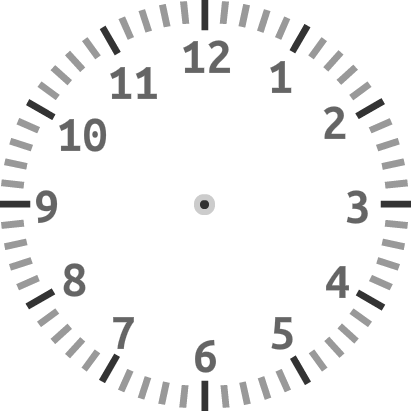
\includegraphics[width=0.3\textwidth]{2-04-1}
\end{figure}

Якщо годинна стрілка стоїть на~2, де вона опиниться через 3~години?
Якщо стоїть на~10, де буде через 5~годин?
На~11, де буде через 18?


\problem
Запиши математичною мовою словесні вирази:
\begin{enumerate}
    \item Число 7 збільшили на~12.
    \item 24 зменшили на~8.
    \item Різниця між числами 5 і~8.
    \item Від 15 забрали 3.
    \item 13 додали до 3.
    \item Сума чисел 7 і~4.
    \item Взяли разом 3 і~5, а~потім додали до суми чисел 7 і~4.
    \item Від різниці чисел 10 і~4 мають забрати різницю чисел 5 і~3.
\end{enumerate}
Яка відповідь вийде у~кожному з~випадків? Обчисли.


\problem
Роздивися математичний вираз:
\[
(4 - 2) + 5 + (7 - 3) - (10 - 3)
\]
\begin{enumerate}
    \item Скільки арифметичних дій (додавань та віднімань)
    треба зробити, щоб отримати відповідь?
    \item Виконай дії у~правильному порядку.
    Окремо запиши кожну дію, що виконав.
    \item Спробуй прочитати та записати цей вираз словами
    (подібно до того, як записані словесні вирази в~попередньому завданні).
\end{enumerate}


\problem
В~понеділок Сашко не встиг придумати 16~завдань з~математики,
з~них 6~--- для Федька, а~решту~--- для Марії та~Іванки порівну.
У~вівторок Сашко не встиг придумати ще 5~завдань,
по~2 для Іванки з~Федьком, а~решту~--- для Марії.
Коли прийшла середа, Сашко захотів придумати
ще по~2 завдання для кожного з~учнів, але знову не встиг.
А~потім настав четвер, у~БеркоШко почалися заняття
і~придумувати завдання з~математики було вже запізно.

Питання:
Скільки всього завдань з~математики не встиг придумати Сашко цього тижня?
Для кого з~учнів Сашко не встиг придумати найбільше завдань?
Чи відрізняється кількість непридуманих завдань для кожної з~дівчат?
Якщо так, то на скільки?
Для кого Сашко не встиг придумати парну, а~для кого непарну кількість завдань?


\problem
Обідали 8~вовченят і~6~зайченят. Було 10~морквин і~8~котлет.
Відомо, що кожна тваринка з'їла те, що їй зазвичай подобається
і~рівно по одній.
Скільки котлет залишилося? А~морквин? Запиши розв'язок охайно та зрозуміло.


\problem
% TAGS: many_solutions
Маша стрибнула в~довжину на 1~метр.
Федьковий результат відрізняється на 23~сантиметри.
На яку відстань стрибнув Федько?


\problem
Знайди і~виправ помилки:
\begin{multicols}{2}
    \begin{enumerate}
        \item $37 + 12 = 50$
        \item $27 - (9 + 3) = 15$
        \item $32 - (11 - 7) = 28$
        \item $11 + 11 + 11 = 44$
        \item $(16 - 8) + 13 = 22$
        \item $(13 + 8) - (13 - 8) = 16$
        \item $(13 + 8) + (13 - 8) = 16$
        \item $(13 - 8) + (13 - 8) = 13$
    \end{enumerate}
\end{multicols}


\problem
Накресли один відрізок довжиною у~стільки сантиметрів, скільки тобі років.
А~другий відрізок~--- скільки років твоєму братикові чи сестричці.
За малюнком визнач, на скільки років ти старший (або молодший).
Запиши розв’язання прикладом.


\problem
Зранку Марія принесла до БеркоШко новорічний подарунок у~червоній коробці.
Всередині було 42~цукерки.
Весь день діти вчились, грались, обідали і~поїли всі цукерки.
Спочатку Марія з’їла 12~цукерок, Федько~--- на~2 більше, ніж Марія,
а~Іванка~--- на~4 менше, ніж Федько.
Потім пригостили меншеньких.
Платонові й~Василькові дісталося по 2~цукерки.
А~Варуся одну цукерку з’їла сама, а~іншу~--- віддала Іванці.

Хто в~БеркоШко з’їв більше цукерок: хлопчики чи дівчатка?
Запиши скорочену умову, зроби малюнок, запиши розв’язок
математичною мовою (прикладами) і~відповідь.


\problem
% TAGS: no_solution
Виріши приклади, запиши проміжну дію:
\begin{multicols}{2}
    \begin{enumerate}
        \item $(22 + 7) - (21 - 13) =$
        \item $(22 - 7) + (21 - 13) =$
        \item $(22 - 7) - (21 + 13) =$
        \item $(22 + 7) + (21 - 13) =$
        \item $(22 - 7) + (21 + 13) =$
        \item $(22 + 7) - (21 + 13) =$
        \item $(22 - 7) - (21 - 13) =$
        \item $(22 + 7) + (21 + 13) =$
    \end{enumerate}
\end{multicols}


\problem
Татусі вирішили зробити дітям гойдалку в~дворі висотою 1~м і~80~см.
Привезли два стовпи-опори довжиною 2~м 40~см.
Якої глибини мають бути ями, щоб вкопати опори для гойдалки?


\problem
Суботнім ранком у~дворі БеркоШко мужики рубали дрова.
Спершу Сергій розрубав 3~колоди, кожну на 4~полінця.
Потім Сашко розрубав ще 4~колоди, кожну також на 4~полінця.
А~Андрій рубав колоди на полінця лише навпіл, розрубав 8~колод.
Потім вони зібрали усі полінця і~склали під лежанкою біля пічки.

Скільки полінець лежить під лежанкою?
Запиши скорочену умову, зроби малюнок,
запиши розв’язок математичною мовою (прикладами) і~відповідь.


\problem
Де трикутників більше?

\begin{figure}[h]
    \centering
    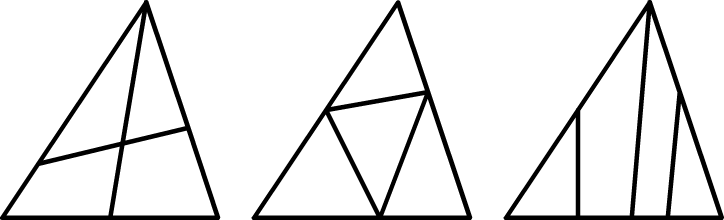
\includegraphics[width=0.6\textwidth]{2-16-1}
\end{figure}


\problem
% TAGS: many_solutions
У~Василька було трохи копійочок.
Якось він знайшов монетку в~10~копійок, а~потім ще п’ятачок.
Він попросив Федька порахувати, скільки в~нього тепер стало грошей,
виявилося, що 59~копійок.
Скільки копійок було у~Василька спочатку?
А~які монетки могли в~нього бути?


\problem
% TAGS: discussion
Аркуш із завданнями забули на столі і~малята заляпали його фарбою так,
що деякі цифри зовсім пропали.
Але ми все-таки спробуємо їх розв’язати.

Порівняй:
\begin{multicols}{2}
    \begin{enumerate}
        \item $25 + 5\hiddendigit \ \square \ 50$
        \item $7\hiddendigit - 11 \ \square \ 50$
        \item $65 + \hiddendigit\hiddendigit \ \square \ 50$
        \item $44 - \hiddendigit \ \square \ 50$
        \item $72 + \hiddendigit\hiddendigit \ \square \ 50$
        \item $28 + 1\hiddendigit \ \square \ 50$
        \item $21 - \hiddendigit \ \square \ 50$
        \item $66 - 3\hiddendigit \ \square \ 50$
    \end{enumerate}
\end{multicols}


\problem
Андрій стрибає в довжину з~місця на 1~м 90~см.
А~хотів би стрибнути на 2~м 60~см.
Наскільки далі потрібно навчитися стрибати Андрієві?


\problem
Знайди якомога більше розгорток кубика на рисунку~\ref{fig:cubes}.

\begin{figure}[h]
    \centering
    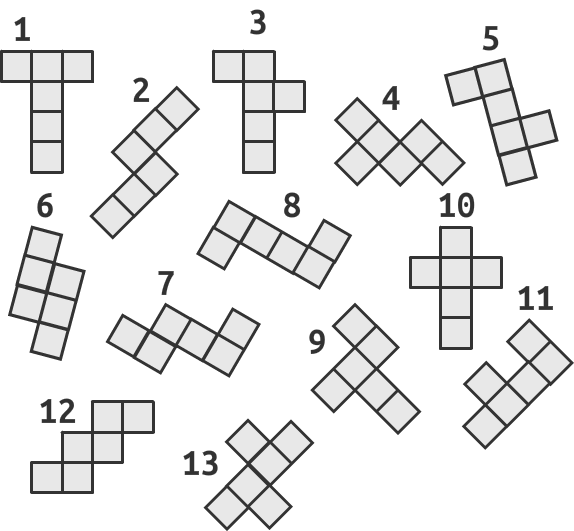
\includegraphics[width=0.6\textwidth]{2-20-1}
    \caption{Можливі розгортки кубика.}
    \label{fig:cubes}
\end{figure}


\problem
На обід у~БеркоШко насмажили 32~котлетки.
Марія, Федько, Іванка, Оля, Катя, Олеся і~Валя з’їли по 2~котлети,
а~Василько, Платон і~Варуся~--- по~1.
На скільки менше котлет залишилось, ніж з’їли за обідом?


\problem
Скільки тобі років?
А~скільки років твоєму братикові чи сестричці?
Скільки років буде тобі, коли твій братик/сестричка стане такий, як ти?


\problem
Яке число знаходиться посередині між:
\begin{multicols}{3}
    \begin{enumerate}
        \item 3 і 5
        \item 7 і 12
        \item 8 і 14
    \end{enumerate}
\end{multicols}


\problem
Скільки горіхів та на яку шальку треба покласти (або забрати),
щоб врівноважити терези, якщо:
\begin{itemize}
    \item на лівій шальці 19~горіхів, на правій~--- 13?
    \item на лівій 12, на правій~--- 24?
    \item на лівій 8, на правій~--- 27?
\end{itemize}


\problem
% TAGS: discussion
Ділення:
\begin{enumerate}
    \item 20~яблук розділи між 4~людьми.
    \item 23~олівці розподіли між 3~людьми.
    \item З~16~клітинок склади 4~однакових квадрата.
    \item 9~кошенят треба роздати 4~хлопчикам.
    \item На тарілці було 27~млинців. 5~учнів з'їли майже всі,
    кожен з'їв однакову кількість.
    Скільки млинців з'їли, скільки залишилось?
    \item У~відрі було 34~стакани компоту.
    За день 6~людей випили майже весь компот,
    кожен випив однакову кількість стаканів компоту.
    Скільки компоту випили, а скільки залишилось?
    \item Склади найбільший прямокутник, використавши
    не~більше 23~клітинок.
    \item Склади найбільший прямокутник, використавши
    не~більше 26~клітинок.
    \item На розв'язання кожного прикладу хлопчик витрачає 7~хвилин.
    Скільки прикладів він зможе розв'язати за годину?
    Скільки часу в~нього залишиться?
\end{enumerate}


\problem
Тарган за 3~хвилини проповз 18~метрів.
Він не зупинявся і~повз весь час, не сповільнюючись і не прискорюючись.
Як думаєш, якої довжини шлях він проповзає за 1~хвилину?
А~за 7~хвилин?


\problem
Спробуй намалювати квадрат, що складається рівно з~2~клітинок.
Якщо вийшло, то чи зможеш ти намалювати квадрат,
що складається рівно з~8~клітинок?


\problem
\problemname{Задача без цифр}
Тато-слон приніс слоненяткові чимало кавунів
і~мама-слониха також трохи принесла.
Слоненя з’їло частину тих кавунів.
Скільки кавунів залишилось?
Виріши задачу без цифр, так, ніби вони відомі, але ти їх не називаєш.


\problem
У~БеркоШко було 4~дітей. Кожний з’їв по 3~оладки.
А~залишилося вдвічі більше, ніж діти з’їли.
Скільки було оладок?


\problem
\problemname{Задача без цифр}
У~Робіна Гуда в~колчані було чимало стріл.
Він прийшов на турнір і~стріляв по мішенях.
В~кожну мішень він влучив однакову кількість разів
і~жодного разу не промахнувся.
Після змагання в~нього залишилося трішки стріл.
Як дізнатися, скільки стріл Робіна влучило в~кожну мішень?
Виріши задачу без цифр, так, ніби вони відомі, але ти їх не називаєш.


\problem
% TAGS: discussion
У більшості випадків речення звичайної мови розповідають про людей, об'єкти,
переповідають думки.
Але бувають речення, що розповідають самі про себе.
Наприклад, ці речення розповідають про себе і~кажуть правду:
\begin{itemize}
    \item Це речення написане українською мовою.
    \item Я придумане Сашком і~надіслане до тебе
    за допомогою комп’ютерної мережі.
\end{itemize}
Ще приклад (з~російської мови):
\begin{itemize}
    \item В~этой фразе двадцать восемь букв.
\end{itemize}
А~от приклад речення, що розповідає про себе, але неправду:
\begin{itemize}
    \item Ти не зміг мене прочитати.
\end{itemize}
Завдання:
\begin{enumerate}
    \item Придумай принаймні 8~речень що розповідають про себе.
    Серед них має бути половина правдивих, а~інша половина~--- неправдивих.
    \item Спробуй придумати правдиве речення про кількість букв
    у~самому собі українською мовою.
    \item Спробуй придумати речення що розповідає саме про себе,
    але не вдається визначити, чи воно правдиве, чи ні.
\end{enumerate}


\problem
В~одній країні стався сильний снігопад~--- за одну ніч
(з~вечора до ранку~--- за 12~годин) випало близько 8~см снігу.
З'ясуй, якщо~б сніг продовжував так само падати і~далі,
то за який час він~би повністю засипав значну частину легкових автомобілів.
(Якщо тобі раптом здалося, що чогось в~умові задачі не~вистачає,
проведи необхідні досліди або вимірювання).


\problem
Які числа можна записати замість букв, щоб рівності стали вірними?
\begin{enumerate}
    \item $(5 + \textit{п}) : 4 = 23$ (і~остача 3)
    \item $25 + (23 - 3 \cdot \textit{к}) \cdot 2 = 47$
\end{enumerate}


\problem
Придумай три приклади, для яких наступне має бути правдою.
\begin{enumerate}
    \item Кожен приклад має складатись з~чотирьох чисел~--- 16, 12, 6, 4,
    поєднаних трьома діями~--- додаванням, відніманням та множенням.
    Якщо потрібно можна використовувати дужки.
    \item В~першому прикладі можна за бажанням або
    спочатку виконати множення або додавання;
    \item В~другому прикладі обов'язково другою дією має
    виконуватися множення (не вийде його виконати першим або останнім);
    \item В~третьому прикладі множення обов'язково має бути останньою дією.
    \item У~всіх трьох прикладах вийде зробити всі обчислення і~отримати відповідь.
\end{enumerate}
Знайди ці відповіді.


\problem
Запиши математичною мовою і~знайди значення виразів:
\begin{enumerate}
    \item різниця чисел 34 і~23;
    \item сума чисел 35 і~27;
    \item різниця чисел 25 і~76;
    \item добуток чисел 3 і~15;
    \item чотири рази по дев'ять;
    \item п'ять десятків і~сім взяли разом із шістьма десятками;
    \item добуток чисел 3 і~4 взяли разом із різницею чисел 7 і~5.
\end{enumerate}


\problem
\problemname{Спостереження за дужками}
У~виразі $10 - 4 + 3 - 2 - 1$ спробували розставити дужки різними способами
і~отримали 9 різних виразів:
\begin{multicols}{2}
    \begin{enumerate}
        \item $(10 - 4) + 3 - 2 - 1$
        \item $10 - (4 + 3) - 2 - 1$
        \item $10 - 4 + (3 - 2) - 1$
        \item $10 - 4 + 3 - (2 - 1)$
        \item $(10 - 4 + 3) - 2 - 1$
        \item $10 - (4 + 3 - 2) - 1$
        \item $10 - 4 + (3 - 2 - 1)$
        \item $(10 - 4 + 3 - 2) - 1$
        \item $10 - (4 + 3 - 2 - 1)$
    \end{enumerate}
\end{multicols}
Виконай дії і~знайди значення кожного з~виразів.
Порівняй отримані відповіді із~значенням початкового виразу,
того, що без дужок.
Виявиться, що від розставлення дужок в~деяких виразах змінилося
значення (відповідь), а~в~деяких~--- залишилося таке саме
як було у~виразі без дужок.
Випиши окремо, на одну сторінку, вирази, де присутність дужок
не~змінила значення, а~на іншу сторінку~--- ті вирази,
де від розставлення дужок відповідь змінилася.
Як думаєш, що спільного в~розташуванні дужок у~виразах,
де відповідь не~змінилася?
А~що спільного в~розташуванні дужок у~виразах на іншій сторінці?
Запиши свої думки-відповіді.


\problem
У~багаторукого Шиви 6~рук і~на кожному пальці~--- каблучка.
Скільки каблучок у~Шиви?


\problem
% TAGS: many_solutions
\problemname{Задача за мотивами гри «Супер фермер»}
Ти маєш 14~кролів, 1~вівцю, 3~поросяти і~3~корови.
Скільки коней і~собак ти можеш виміняти, якщо:
\begin{itemize}
    \item 1~кінь = 2~корови,
    \item 1~корова = 3~свині = великий пес,
    \item 1~свиня = 2~вівці,
    \item 1~вівця = 6~кролів = малий пес.
\end{itemize}
Хто залишиться?


\problem
% TAGS: discussion
\problemname{Ширина фігур (для обговорення)}
Якої найменшої ширини має бути коридор,
щоб через нього зміг пролізти квадратик?
А~який найширший коридор може квадратик перекрити?
Замалюй. Також замалюй найвужчий і~найширший коридор для кола.


\problem
% TAGS: many_solutions
Яке число можна підставити замість букви, щоб рівність стала вірною?
Будь уважним, можливо, в~деяких прикладах замість букви підходить декілька чисел.
\begin{multicols}{2}
    \begin{enumerate}
        \item $А : 12 = 6$
        \item $12 : А = 6$
        \item $12 : А = 1$
        \item $А : 12 = 1$
        \item $А : А = 1$
        \item $А : А = 6$
        \item $А : А = А$
        \item $А \cdot А = А$
    \end{enumerate}
\end{multicols}

\chapter{Третій клас}

\problem
Запиши математичною мовою і знайди значення виразів:
\begin{enumerate}
    \item шість десятків і п'ять взяли разом із трьома десятками і сім;
    \item добуток чисел 7 і 3 взяли разом із різницею чисел 8 і 4;
    \item дочка молодша за маму на 23 роки, а син – молодший на 28 років.
    Хто старший – дочка чи син і на скільки років?
    \item від сімдесяти двох відняти добуток чисел шість і дев'ять;
    \item зменшити дев'яносто чотири на добуток чисел п'ять і сім;
    \item до дванадцяти додати частку від ділення шістдесяти трьох на дев'ять;
    \item різницю чисел 67 і 54 збільшити втричі;
    \item до частки від ділення 27 на 3 додати добуток чисел 6 і 7;
    \item число 112 розділити на різницю чисел 82 і 78;
    \item різницю числа 67 і добутку чисел 12 і 4 збільшити на 54;
    \item суму числа 23 і добутку чисел 4 і 8 зменшити в 5 разів;
    \item суму чисел 13 і 9 розділити на 2;
    \item від різниці чисел 16 і 7 забрати різницю чисел 11 і 3;
    \item суму чисел 63 і 36 зменшити втричі;
    \item добуток чисел 8 і 4 збільшити на 7;
    \item знайти частку від ділення 24 на суму чисел 6 і 2.
\end{enumerate}


\problem
У вірних числових рівностях хтось замалював деякі цифри
\begin{multicols}{2}
    \begin{enumerate}
        \item 2a + 12 = 37
        \item 14 + 1a = 33
        \item 4a – b6 = 32
    \end{enumerate}
\end{multicols}
Спробуй здогадатися які цифри були замальовані.


\problem
В БеркоШко на занятті були присутні 6 учнів і Сашко.
В кожного з них у кишені була однакова кількість цукерок.
Після того як кожен з'їв по одній цукерці,
а Марійка з'їла дві – всі цукерки склали до купи і порахували.
Виявилось що їх там 20 штук.

Знайди, скільки цукерок було на початку в кожного з присутніх.


\problem
Намалюй:
\begin{enumerate}
    \item чотирикутник у якого три сторони однакові,
    а четверта – довша за інші.
    \item чотирикутник у якого три сторони однакові,
    а четверта – коротша за інші.
    \item прямокутник з трьома однаковими сторонами;
    \item чотирикутник у якого всі сторони однакові, але не квадрат;
    \item три різних чотирикутника, що можна скласти рівно з 2 клітинок;
    \item декілька різних прямокутників у яких одна сторона
    на 6 см довша за іншу;
    \item декілька різних прямокутників я яких одна сторона
    в три рази довша за іншу;
    \item прямокутник у якого одна сторона на 6 см довша за іншу
    і водночас втричі довша;
\end{enumerate}


\problem
Вранці в школі в кошику було скількись яблук, частину взяли на компот,
а решту роздали учням порівну.
Як дізнатись, скільки було яблук у кошику, якщо відомо скільки було учнів,
по скільки яблук вони з'їли і скільки пішло на компот.


\problem
Банки:
\begin{enumerate}
    \item Є три банки на 2, 3, і 4 літри. Чотирилітрова банка повна соку.
    Як перелити половину у трилітрову банку?
    \item З повної 4-літрової банки соку необхідно розлити сік 
    у 2 порожні банки, одна з яких 2-літрова, а друга – 3-літрова.
    Розлити необхідно так, щоб у кожній опинилось по 2 літри соку.
\end{enumerate}


\problem
Побудуй:
\begin{enumerate}
    \item на аркуші в клітинку охайний квадратик зі стороною 4 см;
    \item на аркуші в клітинку квадратик зі стороною 2 см і 3 мм;
    \item на нелінованому аркуші квадратик зі стороною 5 см.
\end{enumerate}
Користуватись можна чим завгодно.


\problem
Міста:
\begin{enumerate}
    \item Є три міста: Київ, Одеса, Чернігів.
    Від Києва до Одеси можна доїхати 2 дорогами,
    а від Одеси до Чернігова – трьома.
    Знайти всі можливі варіанти проїзду від Києва до Чернігова через Одесу.
    \item Відстань від Києва до Кіровограда приблизно вдвічі більша
    за відстань від Києва до Чернігова.
    З Києва у Кіровоград можна доїхати приблизно за п'ять з половиною години.
    Як думаєш, скільки часу потрібно на подорож з Чернігова до Кіровограда?
    \item А від Кіровограда до Вінниці їхати приблизно стільки ж,
    скільки від Києва до Кіровограда.
    Як думаєш за скільки часу можна дістатись з Чернігова до Вінниці?
\end{enumerate}


\problem
Годинник показує 7 годин і 15 хвилин.
Намалюй, уявляючи годинник із круглим циферблатом і стрілками:
\begin{enumerate}
    \item який час він покаже через 6 годин і 35 хвилин?
    \item який час він покаже через 3 години і 55 хвилин?
    \item через деякий час годинник показав 1 годину і 5 хвилин.
    Скільки часу пройшло?
\end{enumerate}
Дай відповідь на кожне з питань і намалюй положення стрілок на циферблаті.


\problem
Остача:
% TODO: fix enumeration items
\begin{enumerate}
    \item остача від ділення деякого числа на 8 дорівнює 5,
    а частка дорівнює 7.
    \item знайди число яке ділили («ділене»).
    \item остача від ділення деякого числа на 7 дорівнює 3.
    Яким може бути число що ділили?
\end{enumerate}


\problem
Годинник відбиває час так: повні години за кількістю годин,
а в половину – один раз.
Скільки разів проб’є годинник за час навчання в школі,
якщо заняття розпочались о 9:00, а закінчились – за 5 хвилин до 17:00.


\problem
На кукурудзі мешкала родина неймовірних зелених хробачків.
Родина була чимала, тому жити разом їм було тісно і неймовірні
зелені хробачки переселились на 4 сусідні кукурудзи. Усі, окрім двох.
Переселились купками по 7 неймовірних зелених хробачків на кожну кукурудзу.
Питання: скільки неймовірних зелених хробачків було в родині до переселення?


\problem
Напиши всі можливі числа, які можна записати цифрами 2, 0, 1, 3.
Відсортуй їх від найменшого до найбільшого.


\problem
Посеред холодного південного океану, біля берегів Антарктиди мешкала
зграя пінгвінів. Вдень вони любили грітись на сонечку, а для цього
вистрибувати на велику крижину.

Якось у понеділок на крижину вискочило одночасно 4 родини пінгвінів,
у кожній родині були тато, мама і троє маленьких миленьких пінгвіненят.

У вівторок пінгвіненята так захопливо гралися на крижині,
що до них приєдналися є 7 братиків-пінгвіненят зі своїми батьками
і ще одна дівчинка-пінгвіненятко зі своїми дідусем і бабусею.

А в середу до пінгвінів на крижині приєдналися ще 2 родини.
В одній було двоє діточок і мама з татом, а в другій – 
одне пінгвіненя, мама, тато і бабуся.

На скільки більше ставало пінгвінів на крижині кожного дня:
у вівторок в порівнянні з понеділком і в середу, в порівнянні з вівторком?
У скільки разів більше пінгвінів грілося на крижині у середу, ніж в понеділок?


\problem
Маша йде до школи 12 хвилин, а Федько – 2 хвилини.
У скільки разів більше часу потрібно Машці, щоб дійти до школи?
Скільки разів Федько встигне збігати туди й назад, за той час, що дійде Маша?


\problem
Розпізнавання фігур

Біля кожної фігури познач умови, під які вона підходить:
\begin{enumerate}
    \item має принаймні 4 кути;
    \item не всі сторони рівні;
    \item має тупий кут;
    \item є опуклим багатокутником;
    \item має увігнутий кут;
    \item є правильним багатокутником;
    \item має хоча б 1 прямий кут;
    \item не має кутів.
\end{enumerate}


\problem
Оля випрала рушнички і вивісила їх сушитись у дворі на мотузочці.
Щоб повісити 1 рушник, їй знадобилось 2 прищіпки.
Щоб повісити 3 рушники – 4 прищіпки (одна прищіпка тримала 2 сусідні рушники).
Скільки прищіпок знадобилось Олі для розвішування 9 рушників?


\problem
Лікар накладав Федькові гіпс.
Щоб зробити один оберт навколо руки, лікар витрачав 24 см бинта.
На скільки повних обертів навколо гіпсу вистачить 5-метрового бинта?
Чи вистачить залишку бинта ще на чверть оберта?
А на півоберта?
А на дві третини?
А на три чверті?


\problem
На лавці сиділи дівчата. Раптом Маша помінялась місцями з Томою.
А потім Тома помінялась місцями з Іванкою.
Зрештою вони сиділи на лавці в такому порядку: Маша, Юля, Тома та Іванка.
У якому порядку сиділи дівчата спочатку?


\problem
Задача про равлика, павучка і тарілочку

Равлик і павучок бігають по тарілочці.
Поки равлик проповзає від однієї крапочки до іншої,
павучок встигає оббігти ціле коло. 

Скільки встигне пробігти павучок за той час,
що равлик зробить коло по тарілочці? 

Де опиниться равлик, тоді, коли павучок пробіжить 16 кіл,
якщо відомо з якої точки починав кожний з них? 

Якщо павучок і равлик побігли з однієї точки в різні боки – 
де вони зустрінуться? 

Де опиниться равлик, коли павучок пробіжить 42 кола, якщо відомо
з якої точки починав кожний з них і рухались вони в протилежні боки?


\problem
Прочитай книгу Свена Нордквіста про дідуня Петсона і його кота Фіндуса,
з якими пригодами дідуньо намагався спекти тортик: як забракло борошна,
як збирався в магазин, а колесо у веліка спустило, як загубився ключ
від столярні, як дідуньо з котом намагались його дістати з колодязя,
як відволікали бика і лізли на горище і таке інше.

Замалюй послідовність цих пригод.


\problem
Одного дня біля школи зібрались Клим, Машка з Платоном, Юля і Тома,
Діма, Іванка і Федько з Васильком. І почали грати у сніжки.

Розділились на дві команди. В одну команду потрапити всі,
хто живе на Берківці, а ті, хто приїжджають – в іншу.
І кожний заготовив собі по 8 сніжок.

\begin{enumerate}
    \item Скільки сніжок було на початку гри у кожної команди?
    \item Діти довго перекодувались сніжками, поки ті не закінчились.
    І тоді хтось помітив, що рівно половина всіх сніжок влучила у стіну школи.
    Скільки снігових кульок налипло на стіну школи?
\end{enumerate}


\problem
Софія пішла у магазин, щоб купити для школи молока, сметани, яєць і хліба.

Вона купила:

3 пляшки молока по 8 грн 5 коп.

2 пачки сметани по 8 грн 64 коп.

1 десяток яєць за 9 грн 67 коп.

І 2 батона по 4 грн 30 коп.

Скільки всього грошей витратила Софія?


\problem
На канікули учням БеркоШко задали приклади.
121 приклад задав Сашко, а решту – Валя.
Діти зібрали усі приклади і розділили порівну між собою.
Кожному дісталося по 48 прикладів на канікули.
Скільки прикладів задала Валя, якщо учнів було семеро?


\problem
Накресли за схемою зі сторонами світу:
\begin{multicols}{2}
    \begin{enumerate}
        \item 4 кл. на Сх.
        \item 1 кл. на Пн.-Сх.
        \item 1 кл. на Сх.
        \item 1 кл. на Пд.-Сх.
        \item 1 кл. на Сх.
        \item 1 кл. на Пн.-Сх.
        \item 3 кл. на Сх.
        \item 1 кл. на Пд.-Сх.
        \item 1 кл. на Сх.
        \item 1 кл. на Пн.-Сх.
        \item 1 кл. на Сх.
        \item 3 кл. на Пн.
        \item 1 кл. на Пн.-Зх.
        \item 4 кл. на Пн.
        \item 1 кл. на Сх.
        \item 1 кл. на Пн.-Зх.
        \item 4 кл. на Зх.
        \item 1 кл. на Пд.-Зх.
        \item 1 кл. на Сх.
        \item 4 кл. на Пд.
        \item 6 кл. на Зх.
        \item 2 кл. на Пн.
        \item 1 кл. на Зх.
        \item 2 кл. на Пд.
        \item 1 кл. на Пд.-Зх.
        \item 1 кл. на Пд.
        \item 3 кл. на Пд.-Зх.
    \end{enumerate}
\end{multicols}


\problem
Накресли на нелінованому аркуші прямокутник розміром 24х16 см.
Знайди його периметр.
% TODO: enumeration?
а) Розділи його навпіл вздовж коротшої сторони.
Знайди периметр половинки.
Знову розділи навпіл і знайди периметр четвертинки.
Знову навпіл і периметр восьмушки і так далі.
б) Випиши усі отримані значення периметрів в один рядок.
Уважно придивись до послідовності чисел і спробуй передбачити,
якими будуть наступні периметри, якщо продовжувати розділяти прямокутники.


\problem
Замалюй і обчисли:
\begin{multicols}{2}
    \begin{enumerate}
        \item 1/2 + 1/3 
        \item 1/2 – 1/3 
        \item 2/3 – 1/2 
        \item 1/3 – 1/4 
        \item забрати від цілого третинку;
        \item до половинки додати четвертинку;
        \item скласти разом половинку і третинку.
    \end{enumerate}
\end{multicols}


\problem
Аркуш паперу склали, розрізали навпіл, потім ще навпіл, і ще, і ще\ldots
і так шість разів.
Скільки утворилось шматочків?


\problem
Чи можна плавати в басейні шириною 5 м, довжиною 10 м, глибиною 4 м,
якщо в нього налити 15 000 л води? А 150 000 л?


\problem
Продовжи рядок чисел (треба здогадатись, за яким законом утворюється
наступне число з попередніх)
\begin{enumerate}
    \item 1, 5, 9, 13, 17, 21…
    \item 57, 54, 51, 48, 45, 42…
    \item 1, 4, 10, 22, 46, 94…
    \item 1, 18, 4, 16, 7, 14, 10, 12, 13, 10…
    \item 1, 4, 3, 8, 5, 12, 7, 16, 9…
    \item 2, 6, 14, 30, 62…
    \item 2, 3, 5, 9, 17, 33, 65…
    \item 0, 1/2, 1 1/2, 2, 2 1/2, 3, 3 1/2, 4 …
    \item 16, 15 2/3, 15 1/3, 15, 14 2/3, 14 1/3, 13 …
    \item 1, 1 3/4, 2 1/2, 3 1/4, 4, 4 3/4, 5 1/2, 6 1/4 …
    \item 0, 1, 4, 10, 20, 35… 
\end{enumerate}


\problem
Розв’яжи рівняння:
% TODO: correct math expressions (currently fractions deleted)
\begin{multicols}{2}
    \begin{enumerate}
        \item (6 * х – 88) : 2 – 37 = 0
        \item 120 – (х – 8) * 12 = 0
        \item 3 * (х – 2) : 5 – 15 = 0
        \item (х * 4 – 2) : 4 + 1/4 = 1/2
        \item (х * 1/2 + 7) : 3 = 7
        \item (3 * х + 1) : 7 = 6
        \item 1/4 * х + (4 + 128 : 4) * 2 = 78
        \item 2 * х + 1/4 = 1/2 
        \item (х + 1/3) * 2 = 1
        \item (3 * х + 1) : 8 = 1/4
    \end{enumerate}
\end{multicols}


\problem
В Ашані купили 5 лотків яєць.
Половину всіх яєць - для мешканців 5хаток, а решта - на школу.
З тих яєць, що віднесли в школу, одне взяли на досліди і залили оцтом.
А решту - розділили на три дні порівну. Вийшло по 8 яєць на день.
Скільки яєць вміщається в один лоток? 


\problem
Папай-моряк з’їв на сніданок 2 банки шпинату і пішов в гості до своєї
подружки Олівії. Але не зміг навіть вийти з будинку. В нього в дверях
зламався замок. А Папаю дуже хотілось побачитись з Олівією, тому він
з’їв ще 1 банку шпинату і вибив двері. Потім він вирішив затулити
чимось двері, щоб злодії не потрапили до будинку. Він знайшов неподалік
велику брилу, спробував підняти її – не вдалося. Тоді він з’їв ще банку
шпинату і зміг посунути її. Поки Папай штовхав брилу до дверей, йому
довелося їсти шпинат ще тричі. І ось, нарешті, можна вирушати до подружки.

Дорогою Папай помітив двох бабусь в автівці, які ніяк не могли рушити
з місця. Щоб підштовхнути авто, він з’їв ще кілька баночок шпинату.

Але на цьому пригоди не скінчились. За рогом хлопчик намагався зняти
з дерева котеня, але його драбина була закоротка і він ніяк не міг
дотягнутись. Тоді Папай з’їв ще шпинату, стільки, скільки й
за сніданком – і підняв драбину разом із хлопчиком до котеняти.

Вже майже біля самого будинку Олівії, черевик Папая заскочив в тротуарну
решітку і морякові знадобилось 40 хвилин і 2 банки шпинату,
або випростатись звідти.

І вже дзвонячи у двері Олівії, Папай зрозумів, що якби він їв по одній
банці шпинату на день, то того, що він вже з’їв за сьогодні,
вистачило б на 2 тижні.

Скільки шпинату з’їв Папай, поки йшов в гості до Олівії, якщо в одній
банці вміщається 400 г шпинату?
Скільки банок він з’їв щоб підштовхнути бабусь в автівці?


\problem
Юля до школи добирається півгодини,
третину цього часу вона їде тролейбусом, решту – йде пішки.
Скільки часу Юля їде тролейбусом?


\problem
Маша збиралась до БеркоШколи і приміряла одяг.
Але довго не могла обрати в чому піти.
За 20 хвилин вона встигла переміряти 4 платтячка, джинси, 3 пари шкарпеток,
спідничку, кофтинку і 7 футболок.
З якою швидкістю Маша встигала перевдягатись,
якщо кожну одежинку рахувати окремо?


\problem
Федько зробив індіанський лук і стріли до нього.
Сів на горісі і почав випускати стріли по мішені.
Він неперервно стріляв 17 хвилин і за цей час випустив 51 стрілу.
А Василько тим часом бігав навколо і шукав в траві випущені Федьком стріли,
знайшов тільки 34.
Визначте швидкострільність  Федька і швидкість з якою Василько
відшукував стріли.


\problem
Іванка прийшла на день народження до Марка рівно о шостій вечора.
На столі стояв іменинний торт, розрізаний на 24 шматочки.
Іванка з’їла один шматочок і цей торт їй надзвичайно сподобався.
Тоді вона пригостилась ще шматочком, і ще одним… а далі вона вже не рахувала.
Тільки коли наїлася, зрозуміла, що сама з’їла третину торта.
Вона глянула на годинник – 19:20.
«О, ще купа часу!» - подумала Іванка і пішла гратись з Марком.
Але дорогою додому її зацікавило, з якою швидкістю вона того
вечора наминала шматочки торта. Порахуйте і ви.


\problem
Минуло 20 років. Клим виріс, став археологом і поїхав у Південну Африку
на розкопки. Одного спекотного дня він натрапив на велику кістку
древньої істоти, ретельно викопав її, поруч була ще одна, і ще, і ще…
До смеркання він викопав 357 кісток. І тільки тут усвідомив, що весь
цей час працював без перерви і навіть не обідав. Він полишив роботу
і повернувся в табір. Дізнайтесь, з якою швидкістю Клим робив розкопки,
якщо того дня він почав роботу об 11:30, а завершив о пів на сьому вечора.


\problem
Діма сплів мотузку довжиною 27 метрів, з них 9 метрів – тільки за сьогодні.
Яку частину мотузки сплів сьогодні Діма?


\problem
Тома читала братику Феді книжку впродовж 25 хвилин,
з них 10 хвилин Федя сміявся.
Яку частину всього часу сміявся Томчин братик?

\chapter{Четвертий клас}

\problem
Розділи торти порівну на всіх запрошених:
\begin{enumerate}
    \item 6~тортів на 48~гостей;
    \item 8~тортів на 48~гостей;
    \item 9~тортів на 108~гостей;
    \item 15~тортів на 120~гостей.
\end{enumerate}


\problem
У~кожного учня в~БеркоШко є: зошити в~клітинку~--- з~математики,
з~живого світу і~два зошити з~англійської, зошити в~лінійку~--- 
з~російської і~української мови, а~також альбоми з~музики і~дослідів.
Скільки зошитів у~всіх учнів БеркоШко разом?


\problem
Валя замовила футболки для Варі, Макса, Росави~--- бо їм не~дісталось навесні,
а~також для Федька, Машки і~Сашка, бо вони свої за літо зносили або загубили :)
За всі футболки разом вона заплатила 696~грн.
Скільки коштує друк однієї футболки? 


\problem
Бабуся в’язала шкарпетки бійцям добровольчого батальйону.
Спершу плела з~синіх ниток, а~коли сині закінчились, почала плести коричневі.
За два тижні вона встигла сплести 14~пар шкарпеток.
\begin{enumerate}
    \item З~якою швидкістю бабуся в’яже шкарпетки? 
    \item Скільки шкарпеток (скільки штук) синього кольору сплела бабуся,
    якщо вона помітила, що коричневих вийшла рівно четвертинка.
\end{enumerate}


\problem
Визнач відстані:

\begin{tabular}{|c|c|c|}
    \hline
    Відрізок & Приблизно, см & Точно, см \\ \hline
    BC & & \\ \hline
    AE & & \\ \hline
    ED & & \\ \hline
    AF & & \\ \hline
    EF & & \\ \hline
    FD & & \\ \hline
\end{tabular}


\problem
% TODO: meaning of the problem?
Запиши скорочену умову~--- лише те, що необхідне для розв’язання,
зазнач одиниці вимірювання величин в~дужках, пояснення до кожної дії
і~відповідь.

Першою країною, яка почала досліджувати космос був Радянський союз (СРСР),
в~той час Україна була в~його складі. Потім активно долучились США.
Зараз космічні дослідження переважно міжнародні.

Трохи історії перших років космонавтики:
В~1957~році в~космос запустили перший супутник «Спутник-1» (СРСР).
Перша тварина у~космічному просторі~--- собака Лайка на «Спутник-2»
у~1957 році (СРСР).
Першим космонавтом став Юрій Гагарін в~1961~році (СРСР).
Вперше до Місяця долетів корабель «Луна-2» (без людей) у~1959 році,
а~в~1970~році на Місяць доставили перший автоматичний планетохід —
«Луноход-1» (СРСР).
Вперше у~відкритий космос вийшов Олексій Леонов у~1965 році (СРСР).
Першою людиною, що висадилась на Місяць став Ніл Армстронг в~1969~році (США).
Далі було ще багато цікавого~--- польоти до інших планет і~орбітальні станції,
кому цікаво~--- можете почитати детальніше.
Перший український космонавт часів незалежності України~--- Леонід Каденюк.
У~1997~році він літав в~космос у~складі міжнародної команди корабля «Колумбія».
Його завданням було дослідження впливу невагомості на розвиток рослин:
ріпи, сої і моху. Політ тривав 16~днів. У~нього було по 12~рослин кожного виду.
Щодня він обстежував рослини і~результати досліджень записував у~протокол,
про кожну рослинку~--- на 1~сторінку. Наприкінці польоту Леонід Каденюк
написав звіт про вплив невагомості на рослини, який мав 3~розділи.
Перший розділ~--- вступ~--- мав 37~сторінок. Другий розділ містив всі
протоколи досліджень. А~в~третьому розділі були описані висновки~---
на 16~сторінках.
(Насправді, я не~знаю, скільки саме сторінок було у~звіті Леоніда Каденюка,
але сам космонавт, його політ і~дослідження рослин~--- точно були \smiley)


\problem
Виріши рівняння:
\begin{multicols}{2}
    \begin{enumerate}
        \item $4096 = 6194 - x$
        \item $678 - 3x = 597$
        \item $87 - x = x + 37$
        \item $2x + 66 = 117 - x$
        \item $831 - 3x = x + 391$
    \end{enumerate}
\end{multicols}


\problem
\problemname{Задача про авантюриста Джека}

\begin{quote}
\itshape
    -- А~хто такий авантюрист? \\
    -- Слово походить з~французької мови aventure~--- «пригода»,
    або англійської adventure. Але це не будь-яка пригода,
    в~українській і~російській мові воно набуло певного відтінку...
    Зараз зрозумієте.
\end{quote}

Жив собі Джек. І~якось йому спало на думку вирушити на розшуки скарбів,
але у~нього не~було ні~карти, ні~команди, нічого. Тоді він позичив
у~сусідів 20~піастрів і~вирушив в~порт, найматись на корабель.

Як і~всім авантюристам, на початку йому дуже щастило.
У~портовому кабаку він познайомився з капітаном, який саме шукав
матросів на корабель. Подеякували, що саме для пошуку скарбів.
Капітан спершу не хотів брати Джека, але той віддав йому всі свої
гроші і~сказав, що працюватиме просто за харчі, аби його тільки взяли.

Так корабель із капітаном  дванадцятьма матросами, одним з~яких був Джек,
вирушив на пошуки. У~капітана справді знайшлась карта закопаних скарбів,
і~він виявився чесною людиною і~запропонував розділити знахідку по-чесному.
Всім матросам однакові долі, а~капітанові~--- вдвічі більше, бо карта його.
Всі із цим погодились.

4~роки корабель шукачів нишпорив морями та океанами в~пошуках острова
скарбів і~зрештою таки знайшов. Велику скриню, в~якій виявилось
2340 золотих піастрів.

Їх розділили: капітанові~--- 2~долі, 12~матросам~--- по одній:

Ті монети, що не~змогли поділити, кинули в~море~--- на знак вдячності
за сприятливий вітер. І~всі команда вирішила пливти далі у~пошуках пригод,
але Джекові вже дуже кортіло додому. Тому він попрощався, забрав свою
частку скарбу і~зійшов у~найближчому порту. Повертатись додому йому було
через півсвіту, але пощастило домовитись з~кораблем, що вирушав у~його
рідні краї, за 10~піастрів.

Плив Джек дуже довго, майже рік, бо саме настав сезон штормів.
Втім таки дістався додому.

Першим ділом від пішов до сусіда віддати борг.

А~той розказав Джекові, що вирушаючи в~подорож, Джек забув заплатити
ренту за будинок і~всі ці 5~років банк нараховував йому борг.

Спантеличений Джек пішов у~банк, до йому виписали квитанцію на 150~піастрів,
які він мав сплатити негайно, аби не потрапити у~боргову яму.

Джек порахував гроші і~зажурився. Довелося знову позичати у~сусіда.

А~ввечері Джек сидів на ганку свого будинку і~мріяв про те,
яким би мав бути той скарб, щоб йому не довелося знову залазити в~борги\ldots

\begin{quote}
    \itshape
    -- Так от, авантюрист може віддати 5~років свого життя
    на розшуки скарбів, лишившись по тому ні з~чим \smiley
\end{quote}


\problem
Намалюй положення стрілок за підказками:
\begin{enumerate}
    \item пів на восьму
    \item 09:15
    \item за чверть п’ята
    \item 16:55
    \item двадцять хвилин по дев’ятій
    \item двадцять хвилин на дев’яту
    \item перша
    \item за 25 хвилин десята
\end{enumerate}


\problem
На Берківці потрібно було замовити дрова.
В~кожну з~5~хаток 5хаток і~ще у~Рогатий дім потрібно по 4~куб.~м дрів,
а~в~школу~--- 6~куб.~м.
У~самоскид вміщається 6~куб.~м, які коштують 2800~грн.

Скільки машин дрів необхідно замовити? Скільки це коштуватиме? 
Як розподілити дрова між усіма хатками порівну?

Коли привезли першу машину, самоскид скинув дрова на купу і~5~людей
складало дрова в дровітниці. Їм знадобилося 3~години.
Скільки часу знадобиться 3~людям, щоб розкласти таку саму кількість дрів?
А~якщо комусь доведеться працювати насамоті, скільки часу він складатиме дрова?


\problem
Дізнайся довжини мостів в~Києві: Московського, Патона,
мосту закоханих в Маріїнському парку, Залізничного мосту.
Визнач найдовший, найкоротший.
Якщо довжина тролейбуса 18~м, то скільки таких тролейбусів
вміститься на кожному мосту, впритул один за одним?


\problem
Тома прочитала цікаву книжку за 15~днів. В книжці було 315~сторінок.
Потім цю книжку попросила почитати Іванка. Їй книга так сподобалась,
що вона читала кожного дня на 7~сторінок більше, ніж Тома.
Через скільки днів Іванка зможе повернути Томі книжку?


\problem
Виріши нерівності:
\begin{multicols}{2}
    \begin{enumerate}
        \item $9000 : a > 450$
        \item $11 \cdot x > 1870$
        \item $4 \cdot y - 8 <= 100$
        \item $5 \cdot (k + 17) >= 175$
    \end{enumerate}
\end{multicols}


\problem
Підрахувати, скільки хлібу з’їдає твоя родина за тиждень.
Якого розміру поле мала обробити родина, щоб мати хліб на весь рік?
Якщо всередньому родина з~чотирьох осіб: тато, мама і~двоє діток,
з’їдає 4~хлібини на тиждень. Вважаємо, що 1~хлібина важить 1~кг,
а~борошна на неї потрібно 400~г. Вихід борошна із зерна~--- 4/5 його ваги.
А~на одному гектарі вирощують від 10 до 150 центнерів пшениці,
залежно від врожайності ґрунтів і~сприятливості умов.
Приймаємо середній показник по Україні за часів СРСР~---
40~центнерів з~1~гектара.


\problem
Том Сойєр сам міг би пофарбувати паркан за 6~годин,
а~Гекльберрі Фінн~--- за 3~години. Але вони почали фарбувати його вдвох,
одночасно, з~протилежний кінців, назустріч один одному.
Через який час вони зустрінуться, пофарбувавши весь паркан,
довжина якого 120~м?


\problem
Зустрілись у~прерії два ковбої Том і~Джері. Постояли, побалакали та й
роз’їхались кожний на своє ранчо. Том поїхав зі швидкістю vТома на схід,
а~Джері, зі швидкістю на х більшою~--- на захід. Їхали до своїх ранчо
вони однаковий час t. Яка відстань між ранчо Тома і~Джері?

А~тепер обчисли відстань, якщо швидкість Тома 47~м/хв,
у~Джері~--- на 4~м/хв більше, а~роз’їжджались вони 2~години?


\problem
Відстань між двома містом Бурмосиків і~містом Викрутасиків~--- 204~км.
Викрутасики добігають в~гості до Бурмосиків за 6~годин.
За скільки годин доходять в~гості Бурмосики,
якщо їхня швидкість на 22~км/год менша, ніж швидкість Викрутасиків?


\problem
\problemname{Незавершена мандрівка}
Троє хлопців з~містечка Радомишль, що на річці Тетерів, зробили пліт.
І~зібрались вирушити на ньому в~мандри до моря. Запаслись харчами,
теплим одягом, картою, різним інструментом і о~9~ранку відпливли вниз
за течією. Вже опівдні вони пропливли повз село Березці, в якому жила
бабуся одного з~хлопців, а~він знав, що до того села відстань 6~км.
Отже вони могли дізнатись з~якою швидкістю вони сплавляються
і~розрахувати, коли дістануться до моря.

Але не все так сталося, як гадалося. Цього дня тато одного з~хлопців
о~9:00 відплив на своєму катері вверх по течії. Катер був доволі швидкий,
минулого літа на озері його швидкість була 14~км/год.

І~ось, коли відстань між ними (катером і~плотом) становила вже 84~км,
він зрозумів, що хлопці попливли в~мандри і~до вечері додому не встигнуть.
Розвернувся і~поплив їх наздоганяти.

Скільки часу минуло з~відчалювання у~Радомишлі, до того як тато
розвернув човна і~поплив навздогін хлопцям?
Скільки часу він їх наздоганятиме?
Яку відстань встигнуть пропливти хлопці на плоті допоки тато їх не перехопить?


\problem
Прямокутний лист фанери довжиною 5~дм і~шириною 3~дм розпиляли на квадратики,
зі стороною 1~см.
Скільки таких квадратиків вийшло?


\problem
Збираючись в~похід, Макс купив собі новий тент і~для міцності вирішив
обшити його тасьмою. Ширина тенту~--- 6~м, а довжина~--- на 4~м більша.
Скільки метрів тасьми йому знадобиться для цього?


\problem
Вовк пробіг певну відстань за якийсь час.
Лось чверть цього шляху пробіг за час, вдвічі менший.
На скільки швидкість лося менша за швидкість вовка?


\problem
За прогнозом погоди від 1~січня 2015~року, температура повітря вдень
в~Києві складатиме:

\begin{multicols}{2}
    7~січня~--- 0~градусів

    8~січня~--- 0~градусів

    9~січня~--- 0~градусів

    10~січня~--- 2~градуси

    11~січня~--- 3~градуси

    12~січня~--- 4~градуси

    13~січня~--- 3~градуси

    14~січня~--- 2~градуси

    15~січня~--- 2~градуси

    16~січня~--- 4~градуси
\end{multicols}

Яку середню температуру повітря очікують в~Києві з~7 до 16~січня?


\problem
Виріши рівняння:
\begin{multicols}{2}
    \begin{enumerate}
        \item $x : 100 = 0$
        \item $x + 100 = 100$
        \item $x \cdot 100 = 100\,000$
        \item $x - 100 = 100\,000$
    \end{enumerate}
\end{multicols}


\problem
Обчисли:
\begin{enumerate}
    \item $1530 : (12 \cdot 6 - 38) \cdot 15$
    \item $4840 + 12\,903 - 80\,125 : 5$
    \item $(420 \cdot 20 - 210 \cdot 30) : 100 \cdot (600 - 591)$
    \item $(500 \cdot 10 - 500 : 10) \cdot 6 : (1000 - 997)$
\end{enumerate}


\problem
Щомісяця батьки дають хлопчикові 100~грн, з~них 65~грн він витрачає
на проїзд і~смаколики, а~решту відкладає на придбання моделей літачків.
Через який час він назбирає вдосталь грошей, щоб придбати 50~моделей літачків,
кожний з~яких коштує 28~грн.


\problem
Жіночка продає в~метро календарі.
Закупає у~видавництві 12~календарів за 50~грн, а~продає кожний по 5~грн.
Скільки вона заробить, якщо продасть 30~календарів?


\problem
Черепашка з~дитинства мріяла подорожувати. І~ось одного сонячного ранку
вона поклала в~наплечник GPS-навігатор, щоб не заблукати,
і~вирушила в~мандрівку.

Першого дня вона доповзла до лісу і~влаштувалась на ночівлю під крислатим
дубом. Перед сном черепашка визначила за навігатором, що цього дня
проповзла рівно 2645~м.

Другого дня вона мандрувала лісом, шаруділа листям, милувалась сонячними
променями, які пробивались крізь гілля, ласувала ожиною і~суницями.
І~ввечері знову перевірила за навігатором яку~ж відстань вона подолала.
Виявилось, що за другий день вона проповзла рівно стільки~ж,
скільки й за перший.

А~третього дня їй вдалося доповзти до гарного лісового озера,
вона влаштувалась на крутому беріжку і~спробувала визначити тепер
яку відстань вона проповзла, але в~навігаторі щось заглючило
і~він не~показував відстані.

Черепашка засмутилась і~почала натискати на всі кнопочки меню врізнобій
і~раптом навігатор видав повідомлення, що за третій день вона проповзла
на 1740~м менше, ніж за попередні два дні разом.

То як далеко від дому відповзла черепашка?


\problem
Підприємець придбав 18~дюжин стільців по 3000~грн за дюжину.
За перевезення заплатив 800~грн.
Відтак кожний стілець продав за 300~грн.
Скільки він заробив?


\problem
У~коробці 80~сірників, коштує вона 1~грн.
Скільки коштують 2000~сірників?


\problem
Перед тим як їхати з~БеркоШко на музику, Клим і~Макс сіли перекусити курагою.
Макс з’їв вдвічі більше за Клима, а~Клим на 6~куражинок менше за Макса.
Скільки кураги з’їв Клим?


\problem
На яке число треба поділити 22849 так, щоб вийшло 36 і~ще 25 в~остачі?


\problem
По дорозі до школи Клим відшукує воронячі гнізда. Вже нарахував 21~гніздо.
Навесні в~кожному з~них з’явиться в~середньому по 3~вороненятка.
Цікаво, скільки вороненят народиться тут за 5~років?


\problem
Чи можна намалювати хатку, на відриваючи олівця від паперу і~на проводячи
жодну лінію двічі?
З~якої точки варто починати?


\problem
На Великому Пагорбі на сторожі сиділи двоє індіанців.
Орлине Око~--- в~племені ірокезів і~Вертлявий Тхір з~племені делаварів.

Раптом вони помітили на узліссі блідошкірих, які шикувались для нападу.
Кожний з~індіанців побіг попередити своє плем’я.
Табори обох племен розташовані на однаковій відстані від Великого Пагорба~---
5~кілометрів, але делавари дізнались про напад блідолицих через 20~хвилин,
а~ірокези~--- через 30~хвилин.

На скільки Вертлявий Тхір бігає швидше за Орлине Око?


\problem
Збільши у~68~разів частку суми чисел 4893 і~1527 та числа 30.


\problem
Два потяги одночасно виїхали назустріч одне одному.
Швидкість одного 80~км/год, а~другого~--- 7/8 від швидкості першого потяга.
Через 2~години після початку руху їм залишалося проїхати
1/3 початкової відстані.
Скільки кілометрів становила відстань між потягами на початку?


\problem
Який середній вік людей, які перебувають у~БеркоШко просто зараз?


\problem
% TODO: meaning of problem?
Одного дня беркошколярики прийшли до школярики завжди о~9:15.
Знайшли на поличці пісочний годинник на 15 хвилин і~почали відміряти ним час.
Щойно пісок пересипався з~однієї чаші годинника в~іншу,
його знову перевертали, навіть під час занять,
навіть під час великої перерви.
Впродовж дня діти встигли перекинути годинник 27~разів.
І~коли пісок пересипався востаннє, всі пішли додому.
О~котрій годині всі пішли додому того дня?


\problem
Для розписування писанок перед Великоднем Женя попросила всіх понавидувати
вдома яєць і~принести до БеркоШко. Коли всі діти поскладали принесені яйця
в~лоточки, видалося заповнити 4~лотки на десяток яєць і~2~--- на~18.
Ще один лоток на 15~яєць принесла з~собою Женя.
Діти старанно робили писанки, топили віск, обережно малювали писачками,
але декілька яєць все~ж таки виковзнули з~рук і~розбились.
Коли діти закінчили заняття писанкарством, то нарахували 87~готових писанок.
То скільки яєць розбилося?


\problem
Якось Тома, Юля, Клим, Федько, Іванка, Варя, Маша і~Макс гралися
в~індіанців і~випадково знайшли поза школою моток ліски, довжиною 7~м 44~см.
І~вирішили зробити з~неї тетиву для своїх луків.
Як розділити ліску на всіх порівну і~якої довжини тетива вийде у~кожного?

\backmatter
% bibliography, glossary and index would go here.

\end{document}
